\section{caching}

\subsection{memory hierarchy intro}
\input{../caching/memHierarchyIntro}

\subsection{locality}
\input{../caching/localityBasics}

\subsection{one-block cache}
\input{../caching/oneBlockCache}

\subsection{direct mapped caches}
\input{../caching/directMappedIntro}

\begin{frame}{terminology}
    \begin{itemize}
    \item row = set
        \begin{itemize}
        \item preview: change how much is in a row
        \end{itemize}
    \end{itemize}
\end{frame}

\subsection{tag/index/offset for direct mapped caches}
\input{../caching/tioDMIntro}

\subsection{prelim. formulas}
\begin{frame}{Tag-Index-Offset formulas (direct-mapped only)}
\def\arraystretch{1.5}
\begin{tabular}{ll}
$m$ & memory addreses bits \\
$S=2^s$ & number of sets \\
$s$  & (set) index bits \\
$B=2^b$ & block size \\
$b$ & (block) offset bits \\
$t = m - (s+b)$ & tag bits \\
$C = B \times S$ & cache size (if direct-mapped) \\
\end{tabular}
\end{frame}


\subsection{tio for DM: exercise}
\input{../caching/tioDmExercise}

\subsection{simulating a direct mapped cache}
\input{../caching/dmExampleAccess}

\subsection{exercise: direct-mapped cache access}
\input{../caching/dmAccessExercise}

\subsection{on split data/instruction caches and hierarchy}
\usetikzlibrary{arrows.meta,calc,patterns}

\begin{frame}{split caches; multiple cores}
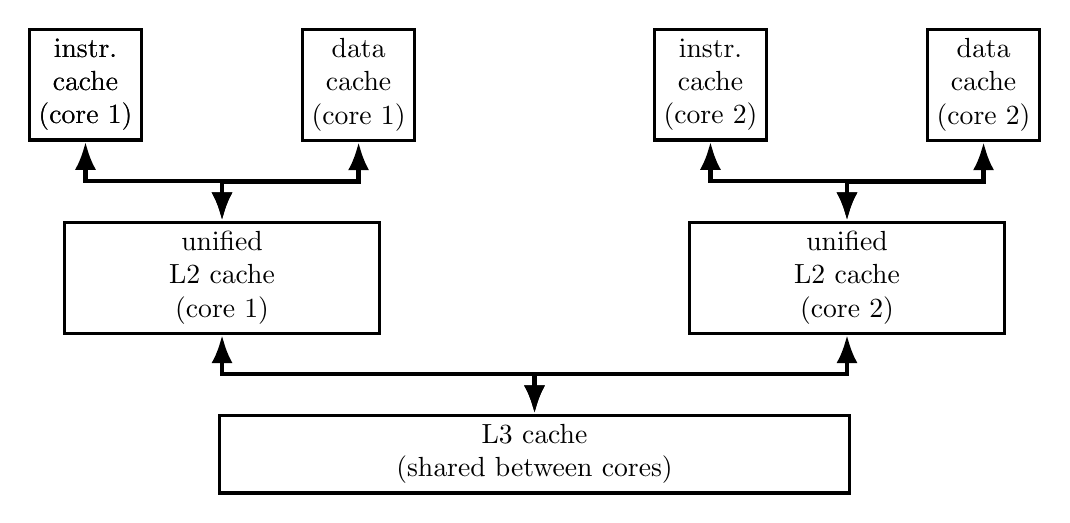
\begin{tikzpicture}
    \tikzset{
        >=Latex,
        connect/.style={<->,ultra thick},
        cache/.style={draw,very thick,align=center},
    }
\node[cache] (icache1) {instr. \\ cache \\ (core 1)};
\node[cache,anchor=west] (dcache1) at ([xshift=2cm]icache1.east) {data \\ cache \\ (core 1)};
\node[cache] (icache2) {instr. \\ cache \\ (core 1)};
\node[cache,anchor=west] (icache2) at ([xshift=3cm]dcache1.east) {instr. \\ cache \\ (core 2)};
\node[cache,anchor=west] (dcache2) at ([xshift=2cm]icache2.east) {data \\ cache \\ (core 2)};
\node[cache, minimum width=4cm,anchor=north] (l21) at ([yshift=-1cm]$(icache1.south)!0.5!(dcache1.south)$) {unified \\ L2 cache \\ (core 1)};
\node[cache, minimum width=4cm,anchor=north] (l22) at ([yshift=-1cm]$(icache2.south)!0.5!(dcache2.south)$) {unified \\ L2 cache \\ (core 2)};
    \node[cache, minimum width=8cm,anchor=north] (l3) at ([yshift=-1cm]$(l21.south)!0.5!(l22.south)$) {L3 cache \\ (shared between cores)};
\foreach \fromC/\toC in {icache1/l21,dcache1/l21,icache2/l22,dcache2/l22,l21/l3,l22/l3} {
\draw[connect] (\fromC.south) -- ++(-0cm,-.5cm) -| (\toC.north);
}
\end{tikzpicture}
\end{frame}

\begin{frame}{hierarchy and instruction/data caches}
    \begin{itemize}
    \item typically separate data and instruction caches for L1
    \vspace{.5cm}
    \item (almost) never going to read instructions as data or vice-versa
    \item avoids instructions evicting data and vice-versa
    \item can optimize instruction cache for different access pattern
    \item easier to build fast caches: that handles less accesses at a time
    \end{itemize}
\end{frame}



% FIXME: direct-mapped and C code example
\section{misses in C, and intuition behind conflicts}
\input{../caching/conflictMissesAndC}

\section{array misses warmup}
\input{../caching/arrayMissesWarmupEx}

\section{array misses warmup, round 2}

\begin{frame}[fragile,label=arrayMissesWarmup4]{C and cache misses (warmup 4)}
\begin{lstlisting}[style=smaller]
int array[8];
...
int even_sum = 0, odd_sum = 0;
even_sum += array[0];
even_sum += array[2];
even_sum += array[4];
even_sum += array[6];
odd_sum += array[1];
odd_sum += array[3];
odd_sum += array[5];
odd_sum += array[7];
\end{lstlisting}
\begin{itemize}
\item {\small
Assume everything but {\tt array} is kept in registers (and the compiler does not do
anything funny).}
\item How many data cache misses on a \textbf{2}-set direct-mapped cache with 8B blocks?
\end{itemize}
\end{frame}

\begin{frame}<0>[fragile,label=arrayMissesWarmup4Answers]{exercise solution}
\newcommand{\mywidth}{0.39}
\begin{tikzpicture}
    \foreach \offset in {-2,-1,0,1,2,...,31,32,33} {
        \draw[black!25,thin] (\offset * \mywidth, 0) rectangle ++(\mywidth, -1);
    }
    \node[font=\large,anchor=east] at (-2 * \mywidth, -.5) {\ldots};
    \node[font=\large,anchor=west] at (34 * \mywidth, -.5) {\ldots};
    \begin{scope}
    \clip (-2.1 * \mywidth, .2) rectangle (34.1 * \mywidth, -1.1);
    \foreach \offset/\name in {8/0,12/1,16/2,20/3,24/4,28/5,32/6} {
        \draw[thin,fill=blue!10] (\offset * \mywidth, 0) rectangle ++(\mywidth * 4, -1)
            node[fill=none,opacity=1.0,black,midway,font=\fontsize{9}{10}\tt\selectfont] {array[\name]};
    }
    \foreach \offset in {-8,0,8,16,24,32} {
        \draw[ultra thick,red!30!black] (\offset * \mywidth, 0)
            rectangle ++(\mywidth * 8, -1);
    }
    \end{scope}
        \draw[very thick, decorate, decoration={brace}] (8 * \mywidth, 0.05) -- ++(8 * \mywidth, 0)
            node[above,midway,align=center,font=\small] {one cache block \\
                                (index 0)};
        \draw[very thick, decorate, decoration={brace}] (16 * \mywidth, 0.05) -- ++(8 * \mywidth, 0)
            node[above,midway,align=center,font=\small] {one cache block \\
                                (index 1)};
        \draw[very thick, decorate, decoration={brace}] (24 * \mywidth, 0.05) -- ++(8 * \mywidth, 0)
            node[above,midway,align=center,font=\small] {one cache block \\
                                (index 0)};
        \draw[very thick, decorate, decoration={brace}] (0 * \mywidth, 0.05) -- ++(8 * \mywidth, 0)
            node[above,midway,align=center,font=\small] {one cache block \\
                                (index 1)};
    \tikzset{
        set both/.style={alt=<2-3>{nodes={fill=red!10}}},
        set 0/.style={
            alt=<2>{nodes={fill=red!10}},
            alt=<3>{opacity=0.1},
        },
        set 1/.style={
            alt=<3>{nodes={fill=red!10}},
            alt=<2>{opacity=0.1},
        },
    }
    \matrix[tight matrix,
        nodes={minimum height=0.5cm,font=\fontsize{8}{9}\selectfont},
        column 1/.append style={nodes={text width=4cm}},
        column 2/.append style={nodes={text width=5cm,font=\fontsize{10}{11}\tt\selectfont,set 0}},
        column 3/.append style={nodes={text width=5cm,font=\fontsize{10}{11}\tt\selectfont,set 1}},
        row 1/.append style={nodes={font=\fontsize{9}{10}\bfseries\selectfont}},
        row 2/.append style={set both},
        row 3/.append style={set 0},
        row 4/.append style={set 1},
        row 5/.append style={set 0},
        row 6/.append style={set 1},
        row 7/.append style={set 0},
        row 8/.append style={set 1},
        row 9/.append style={set 0},
        row 10/.append style={set 1},
        anchor=north west] at (-1, -1) {
        memory access \& set 0 afterwards \& set 1 afterwards \\ 
        --- \& (empty) \& (empty) \\
        read \lstinline|array[0]| (miss) \& \{array[0], array[1]\} \& (empty) \\
        read \lstinline|array[2]| (miss) \& \{array[0], array[1]\} \& \{array[2], array[3]\} \\
        read \lstinline|array[4]| (miss) \& \{array[4], array[5]\} \& \{array[2], array[3]\} \\
        read \lstinline|array[6]| (miss) \& \{array[4], array[5]\} \& \{array[6], array[7]\} \\
        read \lstinline|array[1]| (miss) \& \{array[0], array[1]\} \& \{array[6], array[7]\} \\
        read \lstinline|array[3]| (miss) \& \{array[0], array[1]\} \& \{array[2], array[3]\} \\
        read \lstinline|array[5]| (miss) \& \{array[4], array[5]\} \& \{array[2], array[3]\} \\
        read \lstinline|array[7]| (miss) \& \{array[4], array[5]\} \& \{array[6], array[7]\} \\
    };
\end{tikzpicture}
\end{frame}

\iftoggle{heldback}{}{
\againframe<1-3>{arrayMissesWarmup4Answers}
}


\subsection{mapping misses to sets (DM)}
\input{../caching/setMappingDiagDM}

\subsection{array misses and cache results}
\begin{frame}[fragile,label=arrayMissesWarmup5]{C and cache misses (warmup 5)}
\begin{lstlisting}[style=smaller]
int array[1024]; /* assume aligned */
int even_sum = 0, odd_sum = 0;
even_sum += array[0];
even_sum += array[2];
even_sum += array[512];
even_sum += array[514];
odd_sum += array[1];
odd_sum += array[3];
odd_sum += array[511];
odd_sum += array[513];
\end{lstlisting}
\begin{itemize}
\item {\small
Assume everything but {\tt array} is kept in registers (and the compiler does not do
anything funny).}
\item observation: array[0] and array[512] exactly 2KB apart
\item How many data cache misses on a 2KB direct mapped cache with 16B blocks
\end{itemize}
\end{frame}

\begin{frame}[fragile,label=arrayMissesWarmup6]{C and cache misses (warmup 6)}
\begin{lstlisting}[style=smaller]
int array[1024]; /* assume aligned */
int even_sum = 0, odd_sum = 0;
even_sum += array[0];
even_sum += array[2];
even_sum += array[500];
even_sum += array[502];
odd_sum += array[1];
odd_sum += array[3];
odd_sum += array[501];
odd_sum += array[503];
\end{lstlisting}
\begin{itemize}
\item {\small
Assume everything but {\tt array} is kept in registers (and the compiler does not do
anything funny).}
\item observation: array[0] and array[500] exactly 2KB apart
\item How many data cache misses on a 2KB direct mapped cache with 16B blocks
\end{itemize}
\end{frame}


\section{cache misses on more complex code}
\begin{frame}{actual misses: BST lookups}
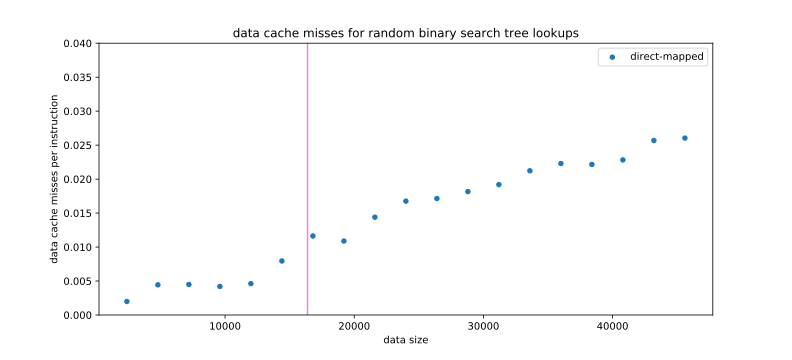
\includegraphics[width=\textwidth]{../caching/bst-one}
\end{frame}

\begin{frame}{actual misses: matrix multiplies}
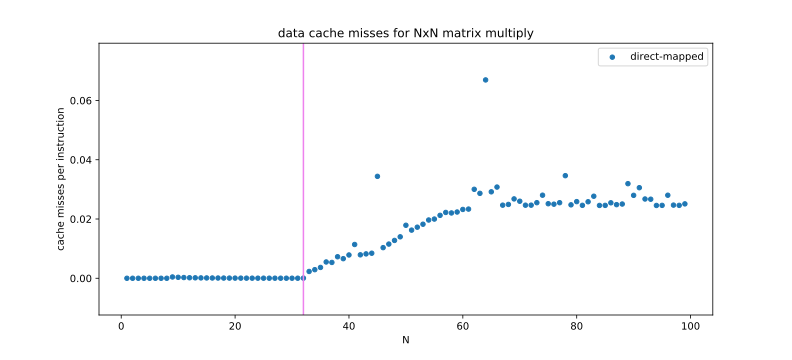
\includegraphics[width=\textwidth]{../caching/mm-one}
\end{frame}


\section{array misses and skipping around}
\begin{frame}<1>[fragile,label=arrayMissesSkip]{misses with skipping}
\begin{lstlisting}
int array1[512]; int array2[512];
...
for (int i = 0; i < 512; i += 1)
    sum += array1[i] * array2[i];
}
\end{lstlisting}
    \begin{itemize}
        \item {\small
    Assume everything but {\tt array1}, {\tt array2} is kept in registers (and the compiler does not do
    anything funny).
        }
    \item
About how many \textit{data cache misses} on a 2KB direct-mapped cache with 16B cache blocks? \\
Hint: depends on relative placement of array1, array2
\end{itemize}
\end{frame}

\begin{frame}{best/worst case}
\begin{itemize}
\item \texttt{array1[i]} and \texttt{array2[i]} always different sets:
    \begin{itemize}
    \item 2 misses every 4 \texttt{i}
    \item = distance from array1 to array2 not multiple of \# sets $\times$ bytes/set
    \end{itemize}
\item \texttt{array1[i]} and \texttt{array2[i]} same sets:
    \begin{itemize}
    \item 2 misses every \texttt{i}
    \item = distance from array1 to array2 is multiple of \# sets $\times$ bytes/set
    \end{itemize}
\end{itemize}
\end{frame}

\begin{frame}{worst case in practice?}
    \begin{itemize}
    \item two rows of matrix?
    \item often sizeof(row) bytes apart
    \item if the row size is multiple of number of sets $\times$ bytes per block, oops!
    \end{itemize}
\end{frame}


\subsection{adding associativity}
%\againframe<13>{pattern1}

\input{../caching/addAssoc}

\subsection{options for replacement}
\input{../caching/replacement}


\subsection{associativity terms}
\input{../caching/assocTerms}

\subsection{tag/index/offset for set-assoc. caches}
\begin{frame}{Tag-Index-Offset formulas}
\def\arraystretch{1.5}
\begin{tabular}{ll}
$m$ & memory addreses bits \\
$E$ & number of blocks per set (``ways'') \\
$S=2^s$ & number of sets \\
$s$  & (set) index bits \\
$B=2^b$ & block size \\
$b$ & (block) offset bits \\
$t = m - (s+b)$ & tag bits \\
$C = B \times S \times E$ & cache size (excluding metadata) \\
\end{tabular}
\end{frame}


\subsection{tag/index/offset exercise}
\subsubsection{setup}
\input{../caching/tioExerciseIntro}
\subsubsection{the exercise}
\input{../caching/tioExercise}

\subsection{mapping misses to sets (DM)}
\input{../caching/setMappingDiag3}


\section{array misses and associative caches?}
\begin{frame}[fragile,label=arrayMissesAssocBig1]{C and cache misses (assoc)}
\begin{lstlisting}[style=smaller]
int array[1024]; /* assume aligned */
int even_sum = 0, odd_sum = 0;
even_sum += array[0];
even_sum += array[2];
even_sum += array[512];
even_sum += array[514];
odd_sum += array[1];
odd_sum += array[3];
odd_sum += array[511];
odd_sum += array[513];
\end{lstlisting}
{\small
Assume everything but {\tt array} is kept in registers (and the compiler does not do
anything funny).\\
opbservation: array[0], array[256], array[512], array[768] in same set}
\begin{itemize}
\item How many data cache misses on a 2KB 2-way set associative cache with 16B blocks
\end{itemize}
\end{frame}

\begin{frame}[fragile,label=arrayMissesAssocBig2]{C and cache misses (assoc)}
\begin{lstlisting}[style=smaller]
int array[1024]; /* assume aligned */
int even_sum = 0, odd_sum = 0;
even_sum += array[0];
even_sum += array[256];
even_sum += array[512];
even_sum += array[768];
odd_sum += array[1];
odd_sum += array[257];
odd_sum += array[513];
odd_sum += array[769];
\end{lstlisting}
{\small
Assume everything but {\tt array} is kept in registers (and the compiler does not do
anything funny).\\
observation: array[0], array[256], array[512], array[768] in same set}
\begin{itemize}
\item How many data cache misses on a 2KB 2-way set associative cache with 16B blocks?
\end{itemize}
\end{frame}


\section{fixing actual misses}
\begin{frame}{simulated misses: BST lookups}
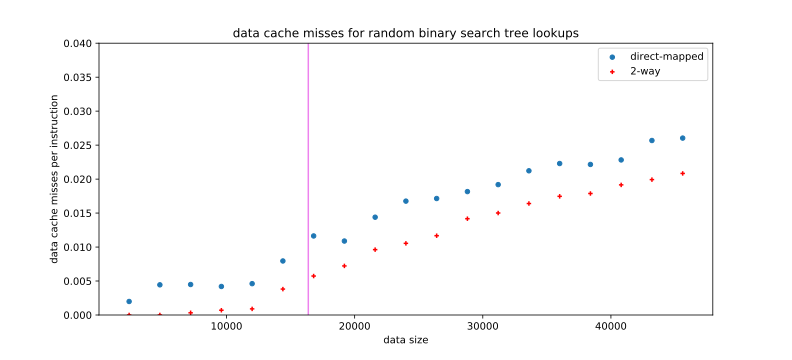
\includegraphics[width=\textwidth]{../caching/bst-both}
\end{frame}

\begin{frame}{simulated misses: matrix multiplies}
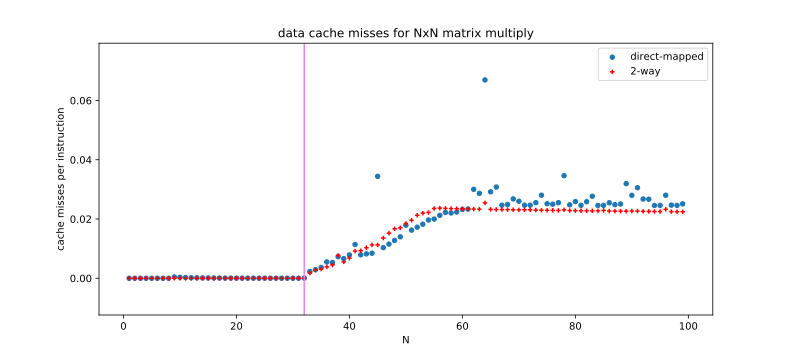
\includegraphics[width=\textwidth]{../caching/mm-both}
\end{frame}


\subsection{options for handling writes}
\input{../caching/writePolicy}

\subsection{exercise: write/replacement policies}
\input{../caching/writeReplaceExercise}

\subsection{fast writes: write buffers}
\input{../caching/fastWrites}

\subsection{miss types}
\begin{frame}{cache miss types}
    \begin{itemize}
        \item common to categorize misses:
            \begin{itemize}
            \item roughly ``cause'' of miss assuming cache block size fixed
            \end{itemize}
        \vspace{.5cm}
        \item \textit{compulsory} (or \textit{cold}) --- \myemph{first time} accessing something
            \begin{itemize}
            \item adding more sets or blocks/set wouldn't change
            \end{itemize}
        \item \textit{conflict} --- sets aren't big/flexible enough
            \begin{itemize}
            \item a fully-associtive (1-set) cache of the same size would have done better
            \end{itemize}
        \item \textit{capacity} --- cache was not big enough
    \end{itemize}
\end{frame}


\section{cache tradeoffs}
\input{../caching/cacheTradeoffs}

\section{TLB}
\input{../vm/twoLevelPtLib}
\subsection{review: page table lookup (1)}
\input{../vm/twoLevelPTAlt}

\subsection{review: page table lookup (2)}
\againframe<7>{twoLevelPtLookup}

\subsection{why cache page table entries?}
\input{../caching/tlbWhy}

\subsection{how TLB fits in page table lookup}
\input{../caching/tlbMulti}

\subsection{how TLBs are organized}
\input{../caching/tlbOrganization} % FIXME: emphasize that AFTER this is normal cache access

\subsection{exercise: splitting for TLBs}
\subsubsection{1}
\input{../caching/tlbSplitEx1}
\subsubsection{2}
\input{../caching/tlbSplitEx2}


\subsection{exercise: TLB access pattern}
\input{../caching/tlbAccessExPrep}
\input{../caching/tlbAccessEx}


\subsection{TLBs and context switches}
\input{../caching/tlbSwitch}

